\subsection{典范余各向同性膜与形变量子化}\label{abranes}

\subsubsection{$A$-膜}\label{aobranes}

现在讨论 $A$-模型的膜。最熟悉的 $A$-膜是拉格朗日膜。拉格朗日 $A$-膜的支撑是 $Y$ 的拉格朗日子流形 $L$。这样的子流形总是中间维的，即若 $\dim Y=2n$，则 $\dim L=n=\frac12\dim Y$。支撑为 $L$ 的 $A$-膜的定义依赖于 $L$ 上 Chan--Paton 丛（简称 $\CP$ 丛）的选取。我们的基本例子是秩 1 的拉格朗日 $A$-膜。

支撑在 $L$ 上的秩 1 $A$-膜的 $\CP$ 丛，通常被描述为带平坦酉联络的复线丛 $\L\to L$。这个描述局部上足够，若 $L$ 是可定向流形并选定了 spin 结构，则整体上也足够；但一般地说它略嫌简化，因为存在一个与膜--$K$-理论关系有关的反常 \cite{FW}。\footnote{\label{anomdesc}这个反常与任何拓扑扭转无关，是 $\sigma$-模型中膜的一般性质。简短说明如下。首先，存在支撑在 $Y$ 上、$\CP$ 丛平凡的膜 $\B_0$。在膜与 $K$-理论的关系中，这个膜对应 $Y$ 上的平凡复线丛。现在考虑任何其它膜 $\B_1$，支撑在某个子流形 $L\subset Y$ 上，$\CP$ 丛为 $\L\to L$。若 $\L$ 秩为 1，则朴素地看它是 $L$ 上的复线丛。然而标准分析表明，$(\B_0,\B_1)$ 系统在 Ramond 扇区的低能态对应取值于 $\L$ 的旋量。要使这样的态存在（注意并未假定 $L$ 是 spin 流形），$\L$ 必须是 $\spinc$ 结构，而不是复线丛。}正确的整体表述是：$\L$ 是 $L$ 上的平坦 $\spinc$ 结构。平坦 $\spinc$ 结构的概念已在第 \ref{gq} 节描述过：若 $\L$ 是 $\spinc$ 结构，则 $\L^2$ 是带联络的普通复线丛，而 $\L$ 的曲率定义为 $\L^2$ 曲率的一半。

除了熟悉的拉格朗日膜，辛流形 $Y$ 的 $A$-模型还可能有其它膜，即 \cite{KO} 发现的所谓余各向同性膜。余各向同性膜的支撑是 $Y$ 的余各向同性子流形\footnote{余各向同性子流形是指局部可由某些 Poisson 交换函数的零点定义的子流形。例如 $Y$ 自身是余各向同性的；此时不需要任何 Poisson 交换函数。另一个极端是拉格朗日子流形 $L$ 为余各向同性。局部上可选坐标使 $\omega_Y=\sum_i\d p_i\d q^i$，而 $L$ 由 $p_1=p_2=\cdots=p_n=0$ 定义。$p_i$ 就是局部定义 $L$ 的 Poisson 交换函数。拉格朗日子流形是维数最小的余各向同性子流形。}，其维数超过 $\frac12\dim Y$。本文主要关心最简单的情形：秩 1、支撑为整个 $Y$ 的余各向同性膜。复辛流形有典则 spin 结构，故在此情形下涉及 spin 的反常无关紧要；支撑为 $Y$ 的膜的 $\CP$ 丛就是复线丛 $\RR$。

在引入支撑于 $Y$ 的余各向同性膜时，我们允许 $\sigma$-模型中存在一个二形式场 $\sB$，通常称为 $B$-场。本文中 $B$-场总是平坦且拓扑平凡的，即 $\sB$ 只是一个闭二形式。正如 \cite{KO} 所解释的，一般地，在辛形式为 $\omega_Y$、二形式场为 $\sB$ 的辛流形 $Y$ 的 $A$-模型中，支撑为 $Y$、$\CP$ 曲率为 $\sF$ 的秩 1 膜成为 $A$-膜的条件是 $I=\omega_Y^{-1}(\sF+\sB)$ 应为 $Y$ 上的可积复结构。最简单的例子恰好出现在本文关心的情况中。若 $Y$ 是复结构为 $I$、全纯二形式为 $\Omega=\omega_J+\i\omega_K$ 的复辛流形，则在 $\omega_Y=\omega_K$ 的 $A$-模型中，取 $\sF+\sB=\omega_J$ 即可解出 $I=\omega_Y^{-1}(\sF+\sB)$。

我们仍有分别选取 $\sF$ 与 $\sB$ 的自由，只要满足 $\sF+\sB=\omega_J$。不同的可能性在如下意义下等价：它们由 $B$-场规范变换相联系。一般地，$\sigma$-模型在把每个膜的 $\CP$ 丛同时张量以任意酉线丛 $\mathcal S$（曲率为 $\sG$，所有膜用同一个 $\mathcal S$）下不变。这诱导每个膜 $\CP$ 曲率的平移 $\sF\to\sF+\sG$，以及补偿性的平移 $\sB\to\sB-\sG$。

本文中一般最方便的选择是 $\sF=0$、$\sB=\omega_J$。$\sF=0$ 的膜的 $\CP$ 丛可以完全平凡，带平凡平坦联络。在辛形式为 $\omega_K$、$B$-场为 $\omega_J$ 的 $A$-模型中，$\CP$ 丛平凡的余各向同性 $A$-膜，就是我们所谓的\textbf{典范余各向同性 $A$-膜}，记作 $\B_\cc$。这类膜在几何 Langlands 对应的规范理论进路 \cite{KW} 中很重要。

若存在曲率为 $\omega_J$ 的酉线丛 $\RR$，则通过 $B$-场规范变换可令 $\sB=0$，从而得到另一种描述：$\B_\cc$ 的 $\CP$ 丛为 $\RR$。事实上这种描述此前已被使用 \cite{KW,GW}，我们将在第 \ref{qcomp} 节看到一个它有用的理由。不过本文中一般更简单的是取 $\B_\cc$ 的 $\CP$ 丛完全平凡、并令 $\sB=\omega_J$。

一般地，在辛形式为 $\omega_Y$、给定 $B$-场的 $A$-模型中，和 $\omega_\C=\omega_Y-\i\sB$ 称为\textbf{复化辛形式}。在目前情形下它是
\be\label{zoffo}\omega_\C=\omega_Y-\i\sB=\omega_K-\i\omega_J=-\i\Omega.\ee

\begin{figure}[htbp]
 \centering
 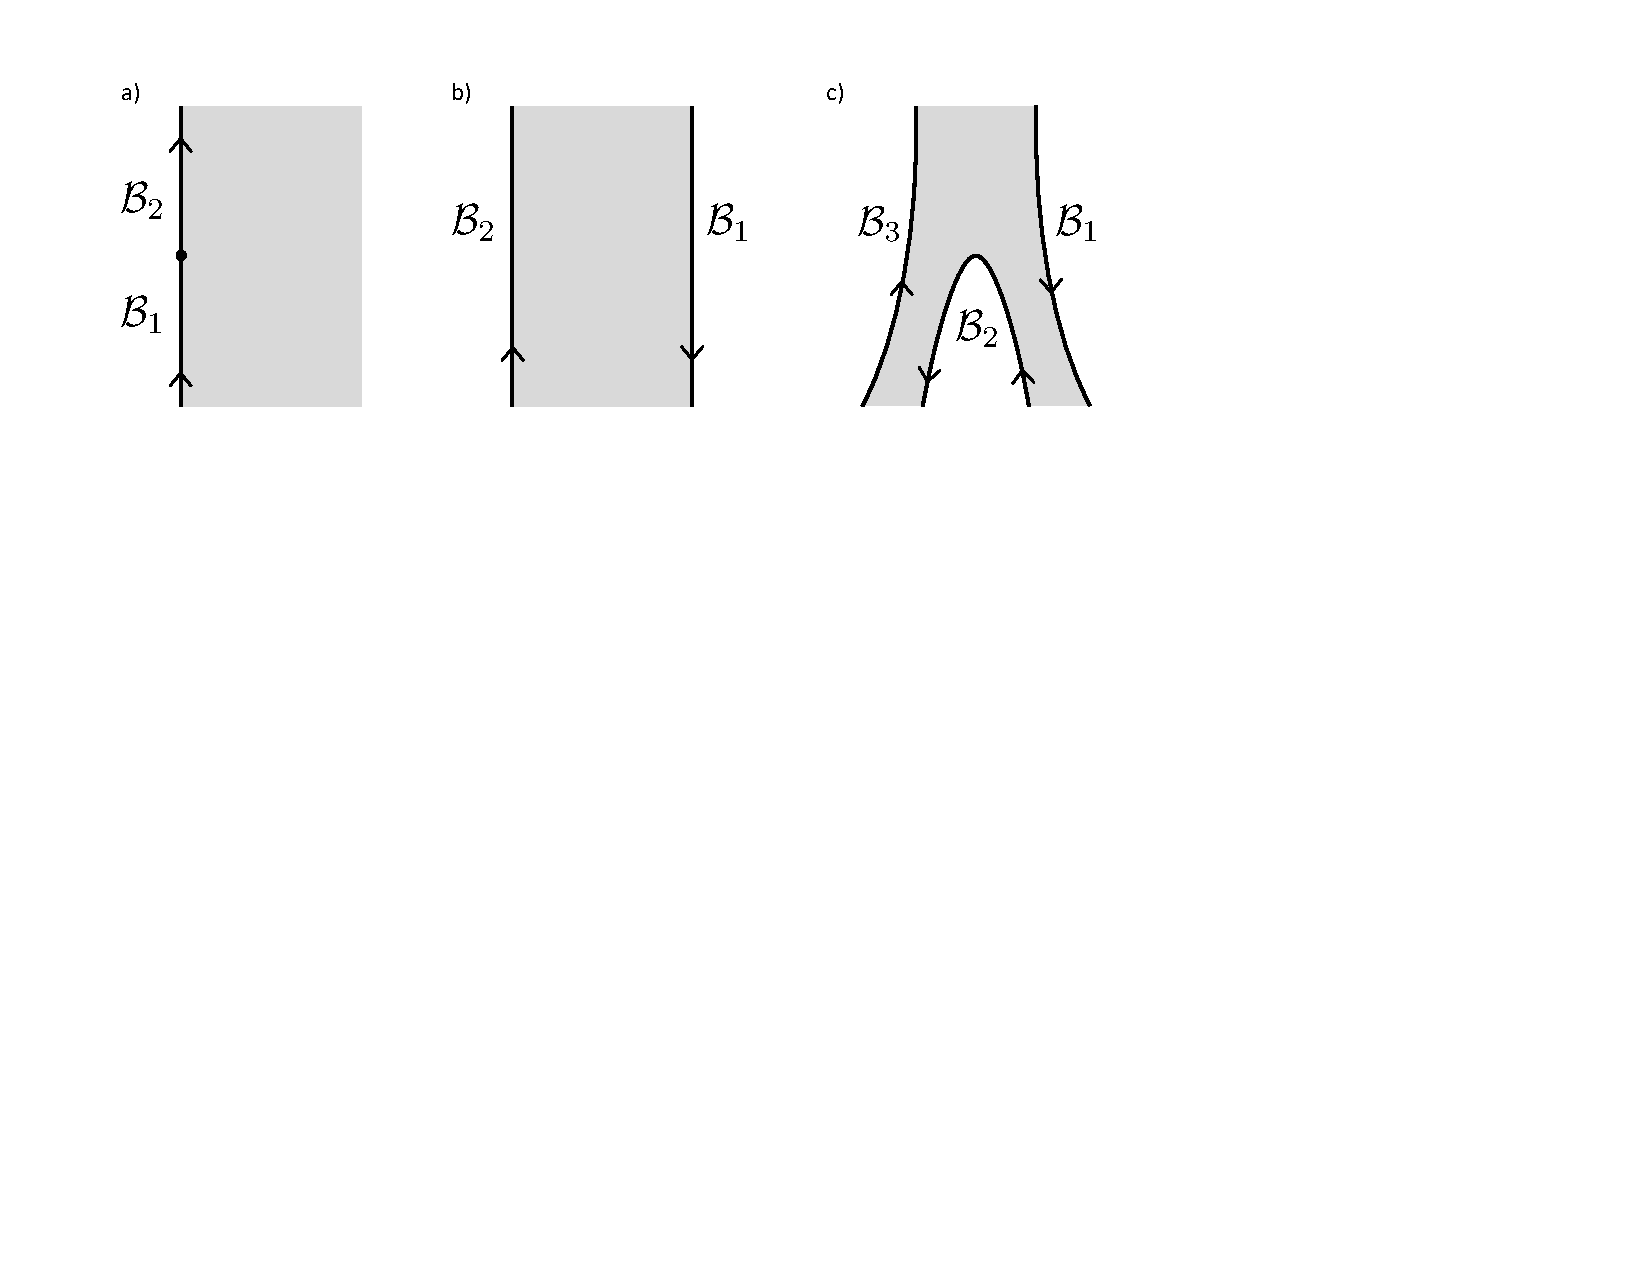
\includegraphics[width=0.86\textwidth]{figures/1_Conventions.pdf}
 \caption{\small (a) 对于二维流形 $\Sigma$ 的左边界，约定“时间”沿箭头方向向上流动，因此 $\B_1$ 在下、$\B_2$ 在上的边界条件衔接表示从 $\B_1$ 到 $\B_2$ 的跃迁，代数上即 $\Hom(\B_1,\B_2)$ 的元素。(b) 通过共形变换可把它映成条带，$\B_2$ 在左、$\B_1$ 在右；图中表示 $\Hom(\B_1,\B_2)$ 的元素从图底部传播到顶部。换一个看法，从顶到底读同一幅图，表示对偶空间 $\Hom(\B_2,\B_1)$ 的元素向下传播。（两种看法可通过平面旋转 $\pi$ 互换，旋转保持定向并交换 $\B_1$ 与 $\B_2$；反射会反转平面定向，不允许。）向上与向下的箭头表示 $\Hom(\B_1,\B_2)$ 对 $\B_2$ 协变、对 $\B_1$ 反变。(c) 态射的自然合成 $\Hom(\B_2,\B_3)\otimes\Hom(\B_1,\B_2)\to\Hom(\B_1,\B_3)$（其中 $\B_1$ 映到 $\B_2$，再映到 $\B_3$）对应此图。}
 \label{explained}
\end{figure}

一般地，若 $\B_1$ 是 $A$-膜，则 $A$-模型中 $(\B_1,\B_1)$ 弦的物理态空间是结合代数 $\A$。若 $\B_2$ 是另一 $A$-膜，则 $(\B_1,\B_2)$ 或 $(\B_2,\B_1)$ 物理态的类似空间是 $\A$-模（确切地说，是右 $\A$-模与左 $\A$-模）。$A$-模型与量子化的联系，来自把这一想法用于 $\B_1=\B_\cc$、$\B_2$ 为拉格朗日膜的情形。为简便，我们沿用数学术语，把 $A$-模型中（任意 $\B_1,\B_2$ 的）$(\B_1,\B_2)$ 物理态空间记作 $\Hom(\B_1,\B_2)$。基本想法是：把 $(\B_1,\B_2)$ 弦与 $(\B_2,\B_3)$ 弦接合成 $(\B_1,\B_3)$ 弦，可描述为态射的合成 $\Hom(\B_2,\B_3)\otimes\Hom(\B_1,\B_2)\to\Hom(\B_1,\B_3)$，其中 $\B_1$ 先映到 $\B_2$，再映到 $\B_3$。一般地，$\Hom(\B_1,\B_2)$ 对 $\B_2$ 协变、对 $\B_1$ 反变。与此相关，若 $\B_1$ 的支撑为 $T_1$、$\CP$ 丛为 $E_1$，$\B_2$ 的支撑为 $T_2$、$\CP$ 丛为 $E_2$，则非常粗略地说，$\Hom(\B_1,\B_2)$ 是 $T_1\cap T_2$ 上取值 $E_1^\vee\otimes E_2$ 的某种截面空间（$E_1^\vee$ 是 $E_1$ 的对偶）。示意地，
\be\label{kogo}\Hom(\B_1,\B_2)\sim \Gamma(T_1\cap T_2, E_1^\vee\otimes E_2).\ee
这是非常示意性的说法，因为我们没有说明允许哪类截面（这依赖于所考虑的膜类型的细节），而且一般而言完整的故事要复杂得多。式 \eqref{kogo} 的要点只在于强调 $E_1$ 取了对偶而 $E_2$ 没有。弦与态射关系的一些约定见图 \ref{explained}。

至少在 $\hbar$ 很小时，加法地有：$\Hom(\B_\cc,\B_\cc)$ 是 $Y$ 的上同调群之直和，
\be\label{poklo}\Hom(\B_\cc,\B_\cc)=\oplus_{r=0}^{\dim_\C Y}H^r(Y,\O),\ee
其中 $\O$ 是 $Y$ 上的平凡复线丛。整数 $r$ 标记上同调类的费米子数或“鬼数”。此结果的推导在附录 \ref{details} 中概述，仿照 \cite{GW} 第 2.2 节。由于弦态相接合（或相乘）时费米子数可加，$r=0$ 的态自身构成一个环。上同调的这一部分因而特别重要。许多有趣例子中 $r>0$ 的上同调实际上消失。

当 $Y$ 是仿射代数簇（由 $\C^N$ 上某些多项式函数的零点定义）时，环 $\Hom(\B_\cc,\B_\cc)$ 特别有意思，我们继续在此情形下讨论。仿射簇的层上同调在 $r>0$ 时消失，故只需考虑 $r=0$ 上同调，它作为向量空间是 $Y$ 上的全纯函数空间。如第 \ref{amo} 节所解释，只考虑关于坐标的多项式函数。在普通乘法下，$Y$ 上的全纯函数构成交换结合环 $\A_0$。但这不是 $\A=\Hom(\B_\cc,\B_\cc)$ 的环结构。相反，如 \cite{KW} 第 11.1 节在若干先前发展 \cite{KO,BrS,Ka,Pe,Gu,AZ} 之后所证明的，也如下文将解释的，$\A$ 是 $\A_0$ 的结合非交换形变。

\subsubsection{与形变量子化的关系}\label{defrel}

此推导的基本想法如下。一般地，$A$-模型由某个底层超对称 $\sigma$-模型构造：选取一个满足 $Q^2=0$ 的超荷 $Q$，并限制到 $Q$-不变的可观测量。由于 $Q^2=0$，$Q$-不变可观测量不受作用量中 $Q$-恰当项 $\{Q,\cdots\}$ 的影响。在二维流形 $\Sigma$ 上，考虑靶为 $Y$ 的 $\sigma$-模型及其映射 $X:\Sigma\to Y$。设 $\omega_\C=\omega-\i\sB$ 为 $A$-模型的复化辛形式。若 $\Sigma$ 无边界，作用量取简单形式
\be\label{simpform}\sI=\int_\Sigma X^*(\omega_\C)+\int_\Sigma\{Q,\cdots\}.\ee
换言之，除 $\omega_\C$ 的拉回外，一切都是 $Q$-恰当的。在我们的设定中 $\omega_\C=-\i\Omega$。因此例如 $\Sigma$ 是以 $S^1$ 为边界的圆盘 $D$ 时，作用量为
\be\label{toldo}\sI=-\i\int_DX^*(\Omega)+\int_D\{Q,\cdots\}.\ee
欧氏号差下 Feynman 积分的被积函数为 $\exp(-\sI)$，故该积分示意地是
\be\label{oldo}\int\D X\cdots\exp\left(\i\int_D\Omega\right)\exp\left(-\int_D\{Q,\cdots\}\right).\ee
（这里 $\D X\cdots$ 指对 $X$ 及其它场的积分。）更一般地，可在圆盘边界上插入算符。这类算符表示 $(\B_\cc,\B_\cc)$ 弦，故对应 $Y$ 上的全纯函数 $f_1,\cdots,f_k$（或后文讨论的高次上同调类）。如第 \ref{uses} 节，在圆盘边界上取点 $r_1,r_2,\cdots,r_k$，并记 $f_i(r_i)=f_i(X(r_i))$。于是，边界标以 $\B_\cc$、带边界算符插入的圆盘上 $A$-模型计算的 Feynman 积分为
\be\label{noldo}\int\D X\cdots\exp\left(\i\int_D\Omega\right)\exp\left(-\int_D\{Q,\cdots\}\right)f_1(r_1)f_2(r_2)\cdots f_k(r_k).\ee

这个积分与 $Y$ 上全纯函数环 $\A_0$ 的形变量子化有关。先描述这个概念。形式上，复流形 $Y$ 上全纯函数环的形变量子化，与第 \ref{uses} 节简述的实辛（或 Poisson）流形的形变量子化相当类似，只是被形变的是全纯函数环。若 $\Omega=\frac12\sum_{i,j}\Omega_{ij}\d y^i\d y^j$（$y^i$ 为 $Y$ 的局部全纯坐标），$\Omega^{ij}$ 为 $\Omega_{ij}$ 的逆矩阵，则全纯函数的 Poisson 括号按通常方式定义为
\be\label{pb}\{f,g\}=\sum_{i,j}\Omega^{ij}\partial_i f\,\partial_j g.\ee
于是在形变环 $\A$ 中，对应全纯函数 $f,g$ 的代数元素 $\h f,\h g$ 满足
\be\label{hb}\h f\h g-\h g\h f=-\i\hbar\h{\{f,g\}}_0+\O(\hbar^2),\ee
其中通过写 $\Omega=\frac{1}{\hbar}\Omega_0$（$\Omega_0$ 固定）引入了形变参数，$\{~,~\}_0$ 是用 $\Omega_0$ 定义的 Poisson 括号。在 $\h f\h g$ 按 $\hbar$ 的展开中，$\hbar^n$ 阶项应是形如 $\partial^k f\partial^{2n-k}g$ 的项之和。

积分 \eqref{noldo} 与形变量子化的关系，最精确的解释见 \cite{W}。首先回忆第 \ref{uses} 节：实辛流形 $M$ 的形变量子化可由对映射 $x:S^1\to M$ 的空间 $\pP$ 的积分描述：
\be\label{pyccl}\bigl\langle f_1f_2\cdots f_k\bigr\rangle=\int_\pP\D x\,\exp\left(\i\int_Dx^*(\omega)\right)f_1(r_1)f_2(r_2)\cdots f_k(r_k).\ee
这里假定 $x:S^1\to M$ 接近常值，并把它的像收缩为 $M$ 中一点，从而延拓为 $x:D\to M$（$D$ 是以 $S^1$ 为边界的圆盘）。$M$ 以 $Y$ 为复化，$\omega=\omega_J$ 解析延拓为 $\Omega$。$\pP$ 的复化是映射 $X:S^1\to Y$ 的空间 $\h\pP$。在形变量子化中，可假定 $X:S^1\to Y$ 接近常值，同样得到同伦意义下的延拓 $X:D\to Y$。函数 $\exp(\i\int_Dx^*(\omega))$ 解析延拓为 $\h\pP$ 上的全纯函数，即 $\exp(\i\int_DX^*(\Omega))$。注意正是这个函数作为因子出现在式 \eqref{oldo} 中，作用量的其余部分是 $Q$-恰当的。$M$ 上适当的光滑函数 $f_1,f_2,\cdots,f_k$ 可解析延拓为 $Y$ 上的全纯函数，仍记作 $f_1,f_2,\cdots,f_k$。形式上，式 \eqref{pyccl} 中的表达式 $\D x\exp(\i\int_Dx^*(\omega))$（$\D x$ 为 Feynman 路径积分测度）是无穷维流形 $\pP$ 上的最高次微分形式。它解析延拓为 $\h\pP$ 上的最高次全纯形式 $\D X\exp(\i\int_DX^*(\Omega))$。要在复流形（这里是无穷维流形 $\h\pP$）上积分最高次全纯形式，需要一个中间维的积分圈。因此例如，若 $\Gamma$ 是 $\h\pP$ 中适当类型的中间维圈，我们或可望使积分
\be\label{pyclo}\int_\Gamma\D X\exp\left(\i\int_DX^*(\Omega)\right)f_1(r_1)f_2(r_2)\cdots f_k(r_k)\ee
有意义。

$\h\pP$ 中中间维圈的一个例子是原来的 $\pP$，即映入 $M\subset Y$ 的映射。取此 $\Gamma$ 时，积分 \eqref{pyclo} 化回 \eqref{pyccl}，给出了理解形变量子化的框架。\cite{W} 所证明的是：边界为 $\B_\cc$、边界上带算符插入的圆盘上的积分 \eqref{noldo}，可解释为取另一个积分圈的积分 \eqref{pyclo}，该圈\footnote{我们马上会讨论，需要作一个修正，因为这个圈并不完全是中间维的。}由那些可延拓为关于复结构 $K$ 全纯的映射 $X:D\to Y$ 的映射 $X:S^1\to Y$ 组成。在使积分 \eqref{pyclo} 有意义的“几乎中间维”圈类中，$\Gamma$ 的选取不影响把该积分与 $Y$ 的形变量子化相联系的论证。此陈述的一个有限维类比是：若 $Z$ 是带最高次全纯形式 $\Omega$ 的复流形，则周期积分 $\int_\Gamma\Omega$ 所满足的微分方程不依赖于圈 $\Gamma\subset Z$ 的选取。

这个简短总结省略了很多，但还有一个细节需要解释，尽管它在本文中没有直接作用。如关于式 \eqref{cycl} 的讨论所解释的，若能使积分 \eqref{pyclo} 有意义，就会得到形变 $\A_0$ 的结合代数 $\A$，以及 $\A$ 上的一个迹。迹是复值线性函数 $\h f\to\la\h f\ra$，满足 $\la\h f\h g\ra=\la\h g\h f\ra$。对光滑流形 $M$，迹的经典极限是与辛测度的积分：$f\to\int_M\frac{\omega^n}{n!}f$，其中 $n=\frac12\dim M$。对带全纯函数 $f$ 的复辛流形 $Y$，这没有如此直接的类比。$\frac{\omega^n}{n!}f$ 最接近的类比是 $\frac{\Omega^n}{n!}f$，它是最高次全纯微分形式；但无法在 $Y$ 上积分 $\frac{\Omega^n}{n!}f$。若使用限制到 $M$ 的积分圈 $\pP$，这没有困难；但若使用与 $\B_\cc$ 相联系的积分圈，就需修改其中一个算符的定义，结果得不到迹。我们主要关心非紧 $Y$，因为若 $Y$ 紧，就没有非常值全纯函数可供量子化。若 $Y$ 非紧，对偶是普通 $\bar\partial$ 上同调与紧支撑 $\bar\partial$ 上同调之间的配对。若 $f_1,\cdots,f_{k-1}$ 是 $Y$ 上的全纯函数，则应取 $f_k\in H^{\dim_\C Y}_{\mathrm{cpct}}(Y,\O)$，即最高次紧支撑 $\bar\partial$ 上同调类。于是式 \eqref{pyclo} 中积分的经典极限是 $\int_Yf_1f_2\cdots f_k\frac{\Omega^n}{n!}$。这是良定义的积分，量子修正也良定义。由式 \eqref{pyclo} 的关联函数，按式 \eqref{woppo} 的算符乘积展开，可构造结合代数 $\A$，它在 $\hbar\to0$ 时约化为全纯函数的交换代数 $\A_0$。但这个代数没有附带迹，因为把其中一个算符取为紧支撑上同调类破坏了循环对称。

\cite{W} 对此点的解释是：由指标定理，与 $\B_\cc$ 相联系的圈 $\Gamma$ 实际上比中间维高 $2n=\dim_\C Y$，故不很适合全纯形式的积分。补偿办法是把其中一个函数 $f_i$ 换成 $(0,2n)$-形式。

\subsubsection{实际形变}\label{actual}

对一般的 $Y$，这个构造给出的是 $\hbar$ 的形式幂级数环上的形变量子化。这对 $A$-模型用于量子化还不够；为此需要能把 $\hbar$ 当作复数。等价地，需要取 $\Omega$ 为 $Y$ 上确定的全纯辛形式。此时我们说 $A$-模型给出了一个\textbf{实际}形变代数 $\A$，而不只是形式形变。如第 \ref{amo} 节所述，其充分条件是：以 $Y$ 为靶的底层量子 $\sigma$-模型（$A$-模型是它的扭转版本）应作为完整的量子场论真正存在。特别地，若 $Y$ 容许完备超 Kähler 度量，则确实如此。

在讨论全纯函数环形变量子化的同一问题时，Kontsevich \cite{K2} 提出：粗略地说，若 $Y$ 可通过添加无穷远除子紧化、且 $\Omega$ 在该除子上有极点，则实际形变存在。Kontsevich 的判据有些类似于如下条件：Tian--Yau 关于完备 Calabi--Yau 度量的定理 \cite{TY} 的超 Kähler 版本会预言 $Y$ 具有完备超 Kähler 度量。（这样的定理似乎只在复维 2 可用，那里 Calabi--Yau 度量自动是超 Kähler 的。）

在 \cite{KW,GW} 讨论的一些重要情形中，可直接证明（无需了解量子 $\sigma$-模型）$\sigma$-模型微扰论在有限步后终止，因此 $A$-模型给出实际形变。这发生在 $Y$ 具有伸缩对称、或至少具有渐近伸缩对称、且 $\hbar$ 按正次数缩放时。

例如，考虑复簇 $x^2+y^2+z^2=\j^2$（式 \eqref{osuc}）。此流形在无穷远处渐近于锥 $x^2+y^2+z^2=0$。它有渐近伸缩对称 $(x,y,z)\to\lambda(x,y,z)$，其中 $\j$ 按次数 1 缩放。取全纯辛形式 $\Omega=\d x\d y/(z\hbar)$，其中 $\hbar$ 也按次数 1 缩放。伸缩对称意味着，在得知可以令 $\hbar=1$ 之后，令 $\hbar=1$ 不会损失任何东西。经典环 $\A_0$ 由 $x,y,z$ 生成，次数均为 1，交换关系如 $xy=yx$，另有附加关系 $x^2+y^2+z^2=\j^2$。形变环在 $x,y,z,\j,\hbar$ 的联合缩放下不变，并有明显的旋转 $x,y,z$ 的 $\SO(3)$ 对称性。综合这些事实可得 \cite{GW}：形变环由 $\h x\h y-\h y\h x=\hbar\h z$ 及其循环置换，以及 $\h x^2+\h y^2+\h z^2=\j^2-\frac14\hbar^2$ 给出，其中只有最后一项的数值系数 $\frac14$ 需要一些分析。这个例子也说明了另两个判据：空间 $Y$ 容许完备超 Kähler 度量（Eguchi--Hanson 度量），并有具备 Kontsevich 所需性质的紧化（即 $\bCP^3$ 中的二次曲面 $x^2+y^2+z^2=w^2$）。类似地可考虑由更高次多项式定义的仿射簇。对复辛流形 $x^n+y^n+z^n=b$（$b$ 为复常数），辛形式为 $\d x\d y/z^{n-1}$，可以发现 $n=3$ 时两个判据都满足，$n>3$ 时都不满足。

复余切丛将在第 \ref{cotangent} 节详细讨论，它们有精确的伸缩对称，因而是具有实际形变的例子，尽管一般认为它们不容许完备超 Kähler 度量。它们确实满足 Kontsevich 的判据。
